% Created 2021-09-11 Sat 08:17
% Intended LaTeX compiler: xelatex
\documentclass[letterpaper]{article}
\usepackage{graphicx}
\usepackage{grffile}
\usepackage{longtable}
\usepackage{wrapfig}
\usepackage{rotating}
\usepackage[normalem]{ulem}
\usepackage{amsmath}
\usepackage{textcomp}
\usepackage{amssymb}
\usepackage{capt-of}
\usepackage{hyperref}
\usepackage[margin=1in]{geometry}
\usepackage{fontspec}
\usepackage{indentfirst}
\setmainfont[ItalicFont = LiberationSans-Italic, BoldFont = LiberationSans-Bold, BoldItalicFont = LiberationSans-BoldItalic]{LiberationSans}
\newfontfamily\NHLight[ItalicFont = LiberationSansNarrow-Italic, BoldFont       = LiberationSansNarrow-Bold, BoldItalicFont = LiberationSansNarrow-BoldItalic]{LiberationSansNarrow}
\newcommand\textrmlf[1]{{\NHLight#1}}
\newcommand\textitlf[1]{{\NHLight\itshape#1}}
\let\textbflf\textrm
\newcommand\textulf[1]{{\NHLight\bfseries#1}}
\newcommand\textuitlf[1]{{\NHLight\bfseries\itshape#1}}
\usepackage{fancyhdr}
\pagestyle{fancy}
\usepackage{titlesec}
\usepackage{titling}
\makeatletter
\lhead{\textbf{\@title}}
\makeatother
\rhead{\textrmlf{Compiled} \today}
\lfoot{\theauthor\ \textbullet \ \textbf{2021-2022}}
\cfoot{}
\rfoot{\textrmlf{Page} \thepage}
\titleformat{\section} {\Large} {\textrmlf{\thesection} {|}} {0.3em} {\textbf}
\titleformat{\subsection} {\large} {\textrmlf{\thesubsection} {|}} {0.2em} {\textbf}
\titleformat{\subsubsection} {\large} {\textrmlf{\thesubsubsection} {|}} {0.1em} {\textbf}
\setlength{\parskip}{0.45em}
\renewcommand\maketitle{}
\author{Houjun Liu}
\date{\today}
\title{Nucleic Acids, DNA, RNA}
\hypersetup{
 pdfauthor={Houjun Liu},
 pdftitle={Nucleic Acids, DNA, RNA},
 pdfkeywords={},
 pdfsubject={},
 pdfcreator={Emacs 27.2 (Org mode 9.4.4)}, 
 pdflang={English}}
\begin{document}

\maketitle


\section{DNA/RNA}
\label{sec:orgccd3a2a}
\subsection{Nucleic Acids}
\label{sec:org29d688f}
d-Oxy Ribone Nucleic Acid: DNA Ribone Nucleic Acid: RNA

\textbf{All nucleic acids are comprised of monomer units that's synthesized
together into polymers.} => Just like
\href{KBhBIO101Carbs.org}{KBhBIO101Carbs} or
\href{KBhBIO101AminoAcids.org}{KBhBIO101AminoAcids}

\subsection{3 basic parts of a Nucleic Acid}
\label{sec:org0d17667}
Two parts of the backbone (phosphate and sugar) + a nitrogenous base
that labels what type of nucleotide this is.

\subsubsection{Backbone}
\label{sec:org92329ff}
\begin{itemize}
\item phosphate group
\item sugar (Ribos => sugar in RNA, di-oxy Ribos => sugar in DNA)=> In
di-oby Ribos: a OH pair is replaced with a hydrogen \textbf{only in one
position.} Hence "di-oxy"
\end{itemize}

\subsubsection{nitrogenous base}
\label{sec:orgb4b08e5}
\begin{itemize}
\item Bases in DNA

\begin{itemize}
\item A, T, G, C
\end{itemize}

\item Bases in RNA

\begin{itemize}
\item A, U, G, C
\end{itemize}
\end{itemize}

\begin{figure}[htbp]
\centering
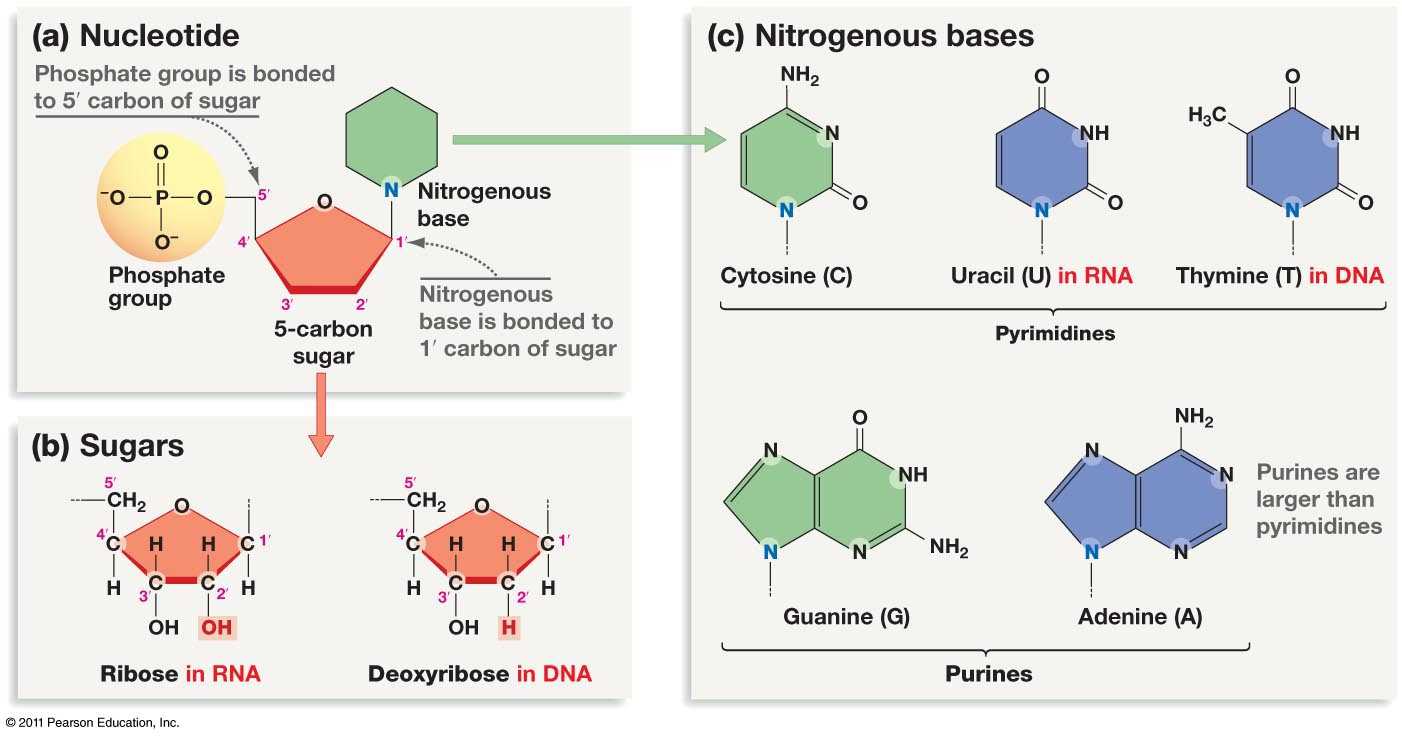
\includegraphics[width=.9\linewidth]{d_na.jpg}
\caption{d\textsubscript{na.jpg}}
\end{figure}

How do we make nucleic acids? Can you guess? Huh? \textbf{Dehydration
synthesis!}

\subsection{Shapes of the DNA}
\label{sec:org49a73f6}
\subsubsection{DNA/RNA Primality}
\label{sec:orga4080c1}
\begin{itemize}
\item 5' => one end of an RNA/DNA part (connection from the phosphate group)
\item 3' => another end of a RNA/DNA part (connection from the third carbon
on the sugar counting from left)
\end{itemize}

\textbf{As in\ldots{}} \begin{center}
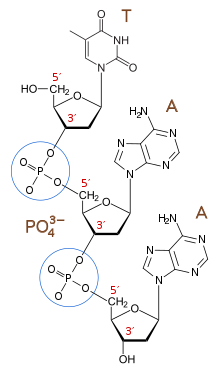
\includegraphics[width=.9\linewidth]{5primeto3prime.png}
\end{center}

\subsubsection{DNA/RNA Strand}
\label{sec:org9aaa87e}
\begin{itemize}
\item DNA is supposed to be double stranded: DNA is \emph{anti-parallel} to each
other => 5' to 3' backbone parallel to 3' to 5' backbone
\item RNA is supposed to be single stranded, but viruses may give them in
bundles so that it would avoid detection
\end{itemize}

See also
\href{KBhBIO101SenseAndAntisense.org}{KBhBIO101SenseAndAntisense}

\textbf{Temp copies of genome is RNA, permanent record in DNA}

\#\# The Central Dogma The process of the central dogma is a rough path by
which DNA is converted into Proteins. This helps us understand how
proteins are made in a cell, and also how viruses could hijack this
process to make themselves.

See \href{KBhBIO101CentralDogma.org}{KBhBIO101CentralDogma}

\subsection{DNA-Made Structures}
\label{sec:org70a2d5a}
In a \href{KBhBIO101Cells.org}{KBhBIO101Cells}, DNA is organized into
different shapes depending on which
\href{KBhBIO101CellLifecycle.org}{KBhBIO101CellLifecycle} that the
cell is in. These structures help facilitate cell replication.

See \href{KBhBIO101DNAStructures.org}{KBhBIO101DNAStructures}
\end{document}
